\documentclass[conference]{IEEEtran}
\IEEEoverridecommandlockouts
% The preceding line is only needed to identify funding in the first footnote. If that is unneeded, please comment it out.
\usepackage{cite}
\usepackage{amsmath,amssymb,amsfonts}
\usepackage{algorithmic}
\usepackage{graphicx}
\usepackage{textcomp}
\usepackage{xcolor}
\def\BibTeX{{\rm B\kern-.05em{\sc i\kern-.025em b}\kern-.08em
    T\kern-.1667em\lower.7ex\hbox{E}\kern-.125emX}}
\begin{document}

\title{Enhancing Image Classification Using Conditional GAN-Based Data Augmentation\\
{\footnotesize Université Paris-Saclay Machine Vision Project}
\thanks{Identify applicable funding agency here. If none, delete this.}
}

\author{\IEEEauthorblockN{Charbel Abi Hana}
\IEEEauthorblockA{\textit{Department of Electrical Engineering} \\
\textit{Université Paris-Saclay}\\
Paris, France \\
charbel-a-h@outlook.com}
}

\maketitle

\begin{abstract}
A major issue in Machine Learning problems is data scarcity. Due to the amount of data obtainable in certain environments we often encounter high variance or overfitting. To deal with overfitting we have many different ways and one of them is to add more data, but this isn't as simple as it sounds sometimes finding more data can be very costly. This is where generating data can be useful, in this project we will be exploring Generative adversarial networks (GANs) for the generation of synthetic data. The goal is to demonstrate that training a classifier on an augmented dataset yields better results than just on small training sets.
\end{abstract}

\begin{IEEEkeywords}
component, formatting, style, styling, insert
\end{IEEEkeywords}

\section{Introduction}
A fundamental bottleneck in machine learning is overfitting, which can be caused by a multitude of reasons. But the major issue in overfitting is usually not enough data, to remedy this we will be exploring a generative adversarial network capable of creating synthetic data which will allow us to add more data to our original dataset. Generative adversarial network(GANs) is a powerful generative model, it transforms the task of learning a data distribution as an adversarial game, which makes it a very good candidate to use in data augmentation. Additionally, it has been shown that GANs can translate images from one context to another in the absence of paired examples\cite{DBLP:journals/corr/ZhuPIE17}.

Using Conditional GANs for data augmentation allows us to translate images as opposed to generating totally new images from noise. GANs are notoriously known to be able to successfully generate outputs far more complex, such as realistic human faces. This suggests that GANs have the potential to successfully augment more complex datasets, such as images.
We thus turned towards Conditional GANs for our data augmentation task, and to test its effectiveness we trained a model using only the small dataset and compared it to the augmented dataset.

\section{Related Work}
It can't be unmentioned that GANs require quite a bit of data to train and reach their full effectiveness making their application to data augmentation impractical, however, research has shown that a generative model can be learned from as little data as a single image \cite{https://doi.org/10.48550/arxiv.1905.01164}. The "SinGAN" learns the coarse features of the images first and gradually moves to fine features, making it possible
to generate images of comparable quality and content to the original. This shows the validity of training generative
models given a small amount of data.
Another method used to address the shortage of data problem can be seen in the realm of machine translation. With a given small dataset of parallel sentences between a source and a target language, translation performance was improved by first training a model on the dataset, using the model to translate additional sentences in the source language, and repeatedly adding the model-translated sentences into the training set to train a new model \cite{https://doi.org/10.48550/arxiv.1909.13151}.
Therefore, we can turn the task of training GANs on the horses and cows data to test the validity of GAN-generated data to augment the original dataset when used to train a classifier. In addition, we will post results of the CycleGAN approach on our training data and inspect the validity of including \textit{translated} data in the training data.

\section{Methods}
In this section we will be explaining the objectives of our GAN and the different model architectures that we used for our data augmentation task.

\subsection{Conditional Generative adversarial network(GANs)}%Change it to urs

We trained a separate GAN to generate images. When training GANs, The model is mainly composed of two parts; First, the generative model, which is mainly to generate images that are as natural and real as possible, second is the discrimination model which mainly judges the authenticity of the image and tries to classify between real and generated images.
\begin{equation}
\min_{G}\max_{D}\mathcal V_{\text{GAN}}\left(D, G \right) = \end{equation}
\begin{align*}
 \mathbb E_{x \sim p_{\text{data}\left( x\right) }}\left[ \log \left\{ D\left( x \right) \right\} \right] + \mathbb E_{z\sim p_{z}\left( z\right)}\left[ \log\left\{ 1 - D\left( G\left( z\right) \right) \right\}\right].   
\end{align*}

where \begin{math}G : R^{100} \longrightarrow R^{16,384}\end{math} maps a noise sample to a 128 × 128 x 3 image and \begin{math}D : R^{16,384} \longrightarrow R\end{math} maps an image to a probability that the image came from the true data distribution (rather than the generator). The discriminator tries to maximize the objective function, so its loss function over all examples is:
\begin{equation}
L_D = - \sum_{x \in \chi, z \in \zeta} \log(D(x)) + \log(1 - D(G(z))) \tag{6}
\end{equation}
The generator can’t affect the first term in the summation, so it tries to minimize the objective function by minimizing its loss:
\begin{equation}
L_G = - \sum_{z \in \zeta} \log(D(G(z)) \tag{7}
\end{equation}
When training a GAN, we ascend the discriminator’s stochastic gradient and descend the generator’s stochastic gradient with respect to \begin{math}\theta_{d}\end{math} and \begin{math}\theta_g\end{math}, respectively, until the losses don’t change anymore. The size of the hidden layers in each GAN are directly proportional to a parameter \begin{math}\alpha\end{math}. In order to combat overconfidence from the discriminator, we use one-sided label smoothing, which penalizes the discriminator for predictions for real images which exceeded .9. To implement this, we simply replace every instance of \begin{math}(1 - D (G (z^i)))\end{math} with \begin{math}(.9 - D (G (z)))\end{math} in the equations above.


\subsection{Model Architecture}
In our Conditional GAN model architecture, we primarily use Convolutional layers as they have a lower number of weights associated with each layer compared to dense layers resulting in higher computational efficiency, conolutional layers output a better spacial and channel-wise representation of images through weights sharing by striding our convolutions. In addition, we use Transpose Convolutional layers to upsample data and generate (128 x 128 x 3) images from noisy vectors. 


\subsubsection{Generator}%Change it to urs
Images were generated starting from a 100-dimensional vector of noise drawn from a standard Gaussian distribution. We used 1 hidden layer with LeakyReLU (with alpha 0.2) which connects to 3 transpose Convolutional layers (128 feature maps with (4, 4) kernels, (2, 2) stride and \textit{same} padding) also with LeakyReLU activation and finally the output is generated through a final Convolutional layer with 3 feature maps representing the RGB channels and (7, 7) kernel with \textit{same} padding and a \textit{tanh} activation function. Letting \begin{math}h^[i]\end{math} denote the input noise, \begin{math}W^{[j]}\end{math} and \begin{math}b^{[i]}\end{math} denoting the weight matrix and the bias vector in the j-th hidden layer, we have
\begin{equation}
h^{[i]} = LeakyRELU(W^{[i-1]}h^{[i-1]}+b{[i-1]})\label{Gen LeakyRELU}
\end{equation}
for i = 1, 2, 3. The size of the hidden layer and the Convolutional layers were designed to grow exponentially between layers while parameterized
by \begin{math}\alpha \end{math}, with h[i] \begin{math}\epsilon R^{16\alpha2^i}\end{math} and we output the vector o \begin{math}\epsilon R^{16,384}\end{math} via
\begin{equation}
o =tanh(W^{[L]}h^{[L]}+b{[L]})
\end{equation}
Where L is the final layer.

\subsubsection{Discriminator}%Change it to urs
The discriminator takes in an image in the form (128 x 128 x 3) matrix where We use 4 hidden layers with LeakyRELU
and dropout (with probability= 0.4), and output a probability that the image is legitimately from the dataset through a final Dense layer with \textit{sigmoid} activation function. Letting \begin{math}h[0]\end{math} denote the input
image, \begin{math}W [j]\end{math} and \begin{math}b[j]\end{math} denoting the weight matrix and the bias vector in the L output layer, we have:
\begin{equation}
o = sigmoid(W^{[L]}h^{[L]}+b{[L]})
\end{equation}


\subsubsection{Classifier}%Change it to urs
The classifier uses3 Convolutional layers with Max-pooling, feature maps going from 50 down to 20 and finally down to 5. ReLU activation function is used for the Convolutional layers as well as kernel size of 3. After flattening the output of the convolutional layers, we pass their output to 2 hidden layers with ReLU activation functions, 30 and 20 (respectively) units. Finally, we obtain the classifier output through a Dense layer with 1 unit and a sigmoid activation function.

%%%%%%%%%%%%%%%%%%%%%%% My edit ends here %%%%%%%%%%%%%%%%%%%%%%%%%%%%%%%%%%%%%%%%%%%%%
\section{Experiments}
\subsection{Dataset}
We're using a dataset composed of Cows and Horses images, where each image has a fixed size of (256 x 256 x 3). The dataset is partitioned into Train/Test splits where we have 82 images in the training set (41 cows images and 41 horses images) and 82 images in the test set. We'll be using the test set to benchmark our classifier performance before and after adding GAN-generated data. It's not crucial to achieve state-of-the-art accuracy on this dataset since the training set is too small. We expect to overfit the classification model easily on such a training set and we wish to highlight through this project the efficacy of adding synthetically generated data through GANs in the training set.
\begin{figure}[htbp]
\centerline{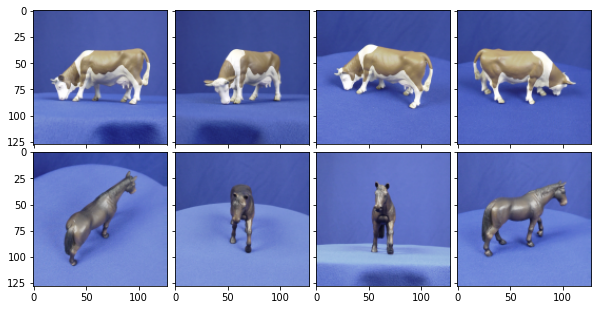
\includegraphics[width=75mm]{1.png}}
\caption{Random Cows and Horses Images from Original Dataset}
\label{fig}
\end{figure}

\subsection{Evaluation Metrics}\label{AA}
We define the following metrics to judge the performance of our classification model; binary-crossentropy loss, accuracy, recall, precision and MSE score. We perform the tests on these metrics for 4 datasets; original dataset (82 images), original + 250 GAN-generated images, original + 500 GAN-generated images, original + 1000 GAN-generated images.

\subsection{Experimentation Details}
For all the experiments, the GANs were trained using Adam optimizer with similar learning rates for the Generator and the Discriminator (0.002). At each training step, we would batch the training dataset with a batch size of 8, generate an image from the random noise vector through the generator model and conditioned labels from the real traninig data (0 for horse and 1 for cow),and using the real labels we can feed the generated output to the discriminator with a ground truth output of a fake image and back-propagate the generator and discriminator errors.
We perform the training for 40000 steps where at each step we train on a random batch of the dataset. In addition, we initialize a Callback where we can visualize the training by generating 8 images, 4 cows and 4 horses.

\subsection{GAN Experimentation Results}
After training the conditional GAN, we notice the difference between outputs generated at 100 steps vs at 35000 steps as shown in figures 2 and 3.
\begin{figure}[htbp]
\centerline{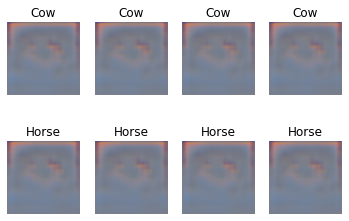
\includegraphics[width=75mm]{2.png}}
\caption{Generated Output after 100 Steps}
\label{fig}
\end{figure}

\begin{figure}[htbp]
\centerline{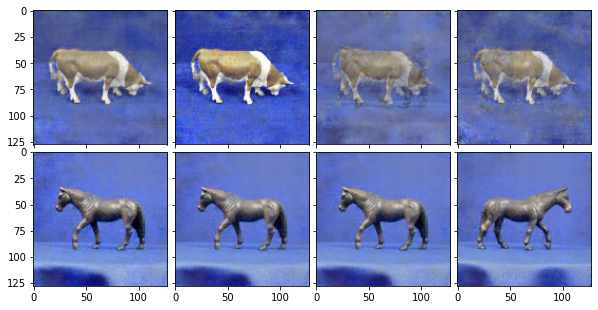
\includegraphics[width=75mm]{3.png}}
\caption{Generated Output after 35000 Steps}
\label{fig}
\end{figure}

For this conditional GAN, we observe the D-loss, G-loss and accuracy from the Discriminator. The D-loss and G-loss formulas are developed above. We notice a lot of variations in the loss data and no discernible convergence of the losses. We plot the following three plots showing the generator loss, discriminator loss and accuracy evolution with the steps.

\begin{figure}[htbp]
\centerline{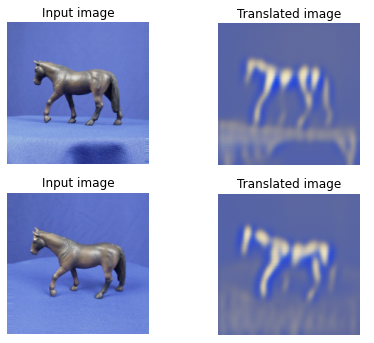
\includegraphics[width=60mm]{5.png}}
\caption{Generated Translated Output after 1 Epoch}
\label{fig}
\end{figure}

\subsection{CycleGAN Experimentation Results}
We train a CycleGAN model with Adam optimizers and a learning rate of 0.0004.A generator with residual layers is implemented. More details of the implementation is shown in the Notebook presented.

In the CycleGAN model we perform the following:
\begin{itemize}
    \item Pass real images through the generators and get the generated images
    \item Pass the generated images back to the generators to check if we can predict the original image from the generated image.
    \item Do an identity mapping of the real images using the generators.
    \item Pass the generated images in 1) to the corresponding discriminators.
    \item Calculate the generators total loss (adverserial + cycle + identity)
    \item Calculate the discriminators loss
    \item Update the weights of the generators
    \item Update the weights of the discriminators
    \item Return the losses in a dictionary.
\end{itemize}

We visualize the following results shown in figure 4 after 1 epoch in contrast to 50 epochs shown in figure 5. 

\begin{figure}[htbp]
\centerline{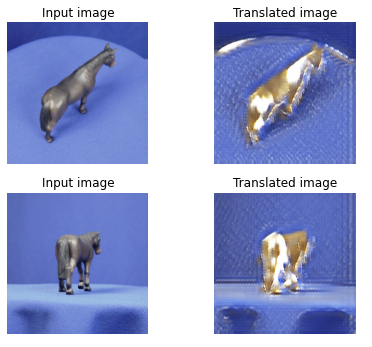
\includegraphics[width=60mm]{4.png}}
\caption{Generated Output after 50 Epochs}
\label{fig}
\end{figure}

\subsection{Classifier Experimentation Results}
For the classifier, we start by training a baseline model on the \textbf{original dataset} for 50 epochs with an Adam optimizer and a learning rate of 0.0001. We obtain the following plots;

\begin{figure}[htbp]
\centerline{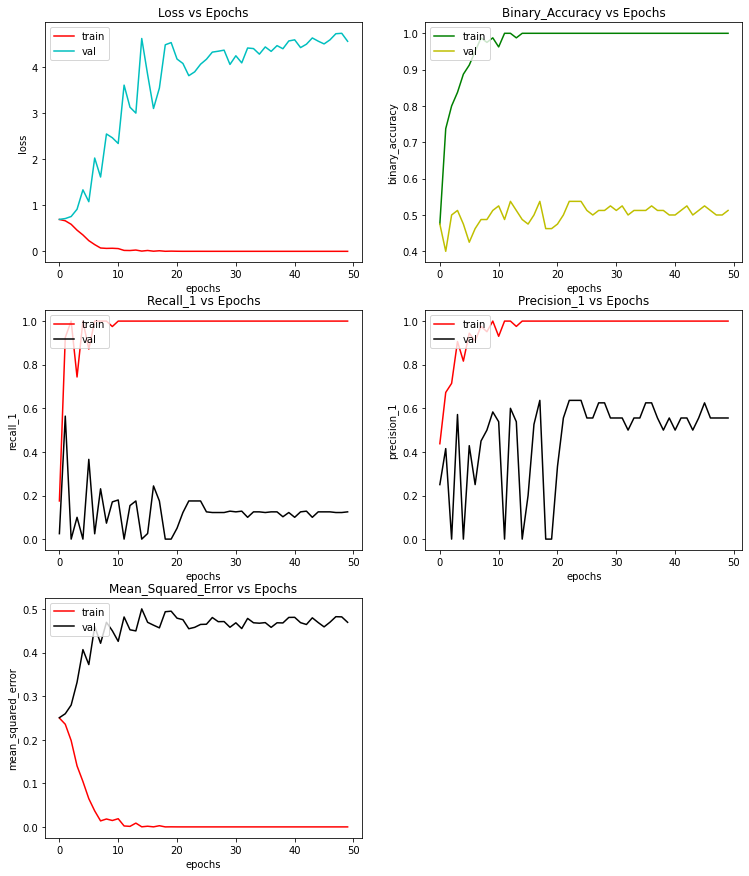
\includegraphics[width=80mm]{plot_orig.png}}
\caption{Classification metrics for classifier trained on \textbf{original dataset}}
\label{fig}
\end{figure}

Training on the original dataset, we clearly see the first indicator of overfitting; a training loss converging and a validation loss diverging or converging with a big loss value difference. The validation set here is the test set, we obtain an accuracy of \textbf{1.0} on the training data however on the validation data we see fluctuations around \textbf{0.5}. The values are somewhat similar for the other metrics.

Training on the \textbf{original+250 GAN-based} yields the results shown in figure 7. In this experiment, we monitor a much more stable validation loss converging at \textbf{0.7} however in this case we can still conclude that the model overfitted the data. The additional data however removed the fluctuations perceived in all the other metrics.

\begin{figure}[htbp]
\centerline{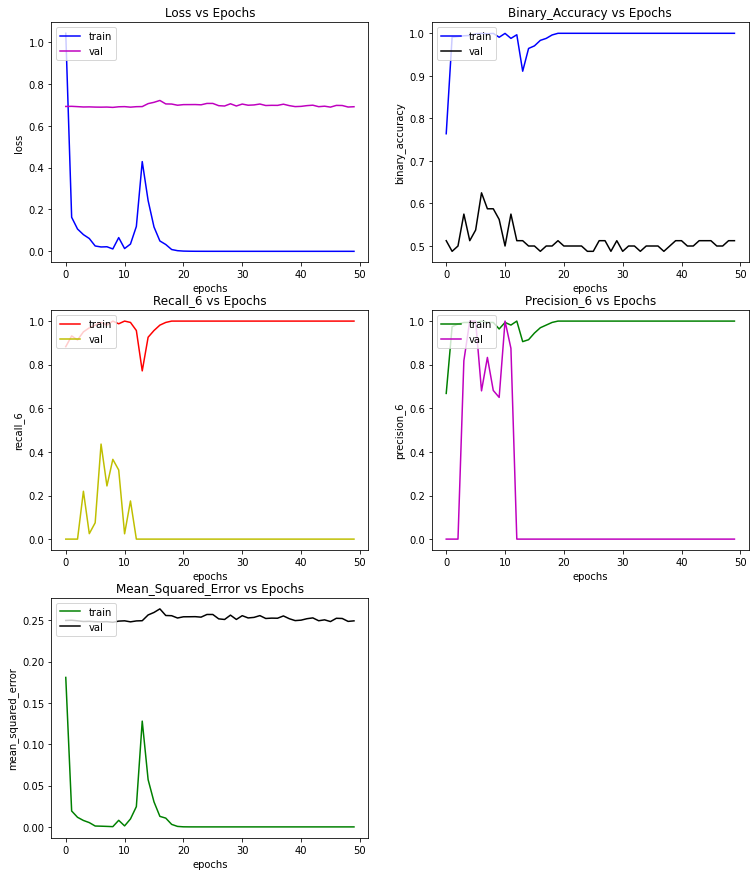
\includegraphics[width=80mm]{plot_250.png}}
\caption{Classification metrics for classifier trained on \textbf{original+250 GAN-based}}
\label{fig}
\end{figure}

Training on the \textbf{original+500 GAN-based} yields the results shown in figure 8. Also, we visualize a better smoothing of the validation metrics while maintaining a validation loss converged at \textbf{0.7}.

\begin{figure}[htbp]
\centerline{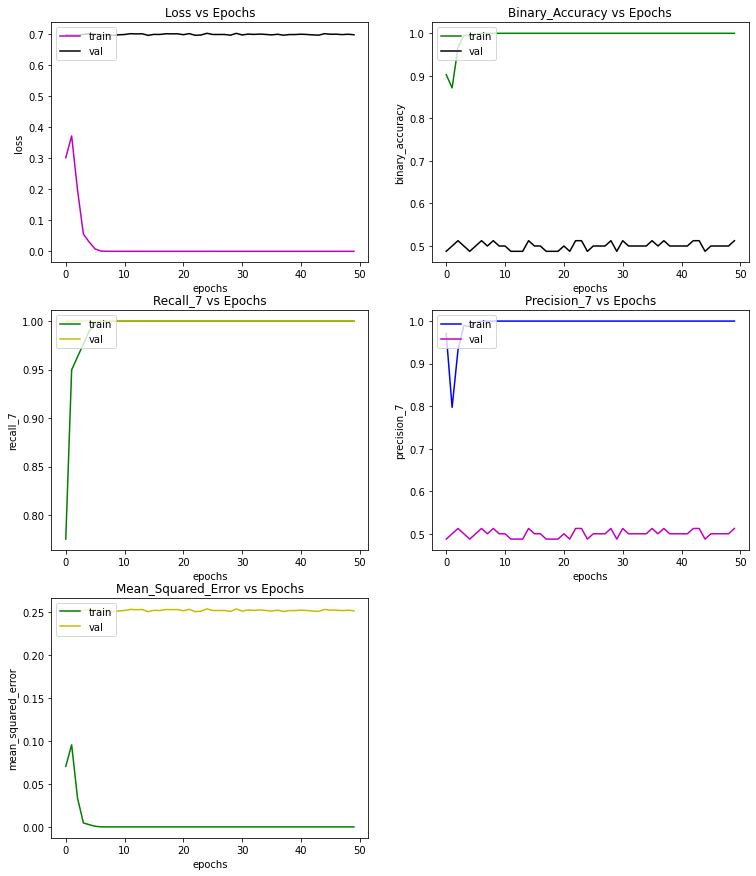
\includegraphics[width=80mm]{plot_500.png}}
\caption{Classification metrics for classifier trained on \textbf{original+250 GAN-based}}
\label{fig}
\end{figure}

Training on the \textbf{original+1000 GAN-based} yields the results shown in figure 9. Training on this number of images showed a fluctuating a high training error indicating we reached a point where our data is too complex for our simple model. This means we generated more data than our model could learn and a method to overcome this is to increase model complexity.

\begin{figure}[htbp]
\centerline{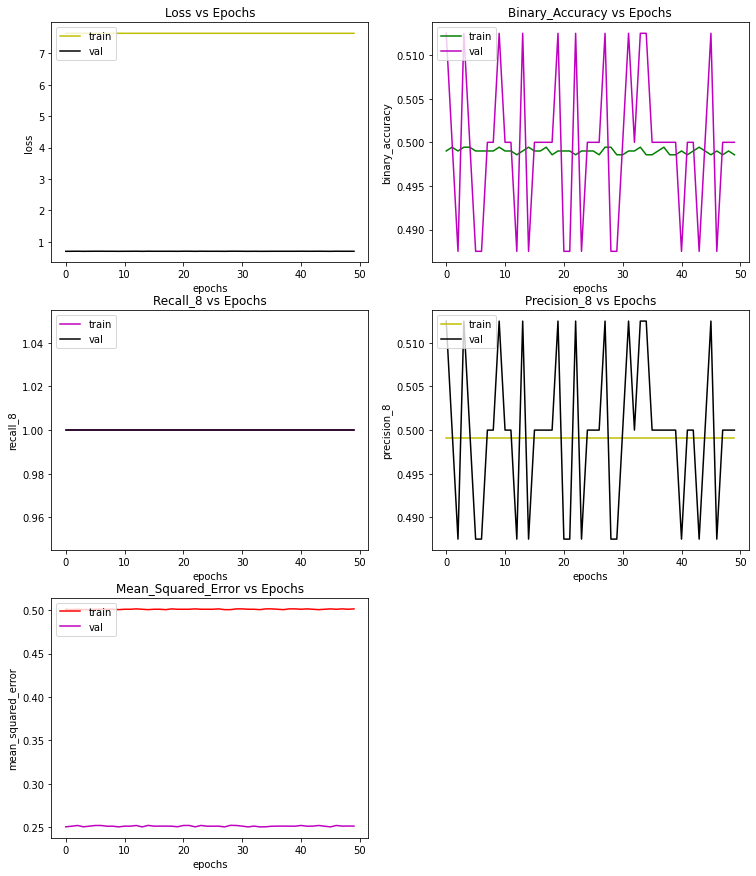
\includegraphics[width=80mm]{plot_1000.png}}
\caption{Classification metrics for classifier trained on \textbf{original+250 GAN-based}}
\label{fig}
\end{figure}

We compile the table shown below to highlight the differences between the losses and the classification metrics between the orignal dataset and the GAN-augmented datasets. 
Of course we should take note that we are generating well above the total number of datapoints in the original dataset. We should later invest in the same methodologies but with bigger datasets giving us the opportunity to tune the ration at which we inject the GAN-generated data.

\begin{table}[h!]
\centering
\begin{tabular}{| *{9}{c|} }
    \hline
\textbf{Metric}    & \multicolumn{2}{c|}{Orig}
            & \multicolumn{2}{c|}{Orig-250-GAN}
                    & \multicolumn{2}{c|}{Orig-500-GAN}
                            & \multicolumn{2}{c|}{Orig-1000-GAN}                \\
    \hline
-   &   \textbf{train}  &   \textbf{val}  &   \textbf{train}  &   \textbf{val}  &   \textbf{train}  &   \textbf{val}  &   \textbf{train}  &   \textbf{val}  \\
    \hline
BCE-Loss   &   0.01  &   5  &   0.01  &   0.7  &  0.01   &  0.7   &   8  &  0.7   \\
    \hline
Accuracy   &    1.0   &     0.5  &   1.0    &     0.6  &   1.0    &    0.5   &   0.5    &   0.5    \\
    \hline
Precision   &   1.0    &   0.1    &   1.0    &    0.5   &   1.0    &    0.5   &   0.5    &    0.5   \\
    \hline
Recall   &    1.0   &    0.5   &    1.0   &   0.4   &    1.0   &    1.0   &    1.0   &  1.0     \\
    \hline

\end{tabular}
\caption{Compiled table of Classification Metrics}
\end{table}

\section{Conclusion}
Throughout this project, we explored GANs training, which showed to be extremely hyper-parameter sensitive. We generated labeled data to augment our small dataset expanding the datapoints from 82 images to 1000+ images with a boost in classification performance. Linked with some regularization methods, we are able to fully develop a proper classifier for this dataset reducing more and more the overfitting effects. We managed to perform this task using Conditional GANs, however, we had to experiment a lot more with DCGANs throughout the practical Notebook where we investigated different Generator/Discriminator architectures and hyperparameters. Finally, we were able to train a Cycle GAN where we can \textit{transfer} between classes (horses and cows) bidirectionally adapting an input image to a target variable. This project has contributed greatly to a hand-on experience using Deep Learning libraries and methodologies like Tensorflow.

\bibliography{citations}

\bibliographystyle{plain} % We choose the "plain" reference style
\bibliography{citations} % Entries are in the refs.bib file
\end{document}
